% This is "sig-alternate.tex" V2.1 April 2013
% This file should be compiled with V2.5 of "sig-alternate.cls" May 2012
%
% This example file demonstrates the use of the 'sig-alternate.cls'
% V2.5 LaTeX2e document class file. It is for those submitting
% articles to ACM Conference Proceedings WHO DO NOT WISH TO
% Strictly ADHERE TO THE SIGS (PUBS-BOARD-ENDORSED) STYLE.
% The 'sig-alternate.cls' file will produce a similar-looking,
% albeit, 'tighter' paper resulting in, invariably, fewer pages.
%
% ----------------------------------------------------------------------------------------------------------------
% This .tex file (and associated .cls V2.5) produces:
%       1) The Permission Statement
%       2) The Conference (location) Info information
%       3) The Copyright Line with ACM data
%       4) NO page numbers
%
% as against the acm_proc_article-sp.cls file which
% does NOT produce 1) thru' 3) above.
%
% Using 'sig-alternate.cls' you have control, however, from within
% the source .tex file, over both the CopyrightYear
% (defaulted to 200X) and the ACM Copyright Data
% (defaulted to X-XXXXX-XX-X/XX/XX).
% e.g.
% \CopyrightYear{2007} will cause 2007 to appear in the copyright line.
% \crdata{0-12345-67-8/90/12} will cause 0-12345-67-8/90/12 to appear in the copyright line.
%
% ---------------------------------------------------------------------------------------------------------------
% This .tex source is an example which *does* use
% the .bib file (from which the .bbl file % is produced).
% TODO REMEMBER HOWEVER: After having produced the .bbl file,
% and prior to final submission, you *NEED* to 'insert'
% your .bbl file into your source .tex file so as to provide
% one 'self-contained' source file.
% ================= IF YOU HAVE QUESTIONS =======================
% Questions regarding the SIGS styles, SIGS policies and
% procedures, Conferences etc. should be sent to
% Adrienne Griscti (griscti@acm.org)
%
% Technical questions _only_ to
% Gerald Murray (murray@hq.acm.org)
% ===============================================================
%
% For tracking purposes - this is V2.0 - May 2012

\documentclass{sig-alternate-05-2015}
  \pdfpagewidth=8.5truein
  \pdfpageheight=11truein
  
  
% Custom package imports
\usepackage[utf8]{inputenc}
\usepackage{microtype}
\usepackage{booktabs}

\usepackage{graphicx}
\usepackage[utf8]{inputenc}
\usepackage{listings}
\usepackage{cleveref}
\usepackage{textcomp}
\usepackage[usenames, dvipsnames]{color}
\usepackage{url}

% Custom config
\graphicspath{{figures/}}

\definecolor{myviolett}{RGB}{127, 0, 85}
\definecolor{darkred}{RGB}{136, 0, 0}
\definecolor{darkblue}{RGB}{52, 89, 127}
\definecolor{lightgreen}{RGB}{44, 55, 0}

\lstset{
	basicstyle=\ttfamily\scriptsize,
	keywordstyle=\color{darkred}\ttfamily,
	stringstyle=\color{darkblue}\ttfamily,
	commentstyle=\color{lightgreen}\ttfamily,
	breaklines=true,
	aboveskip=.75\baselineskip,
	belowskip=1.5\baselineskip,
	upquote=true,
	showstringspaces=false
}

\lstdefinelanguage{dsl} % Farblich orientiert an Eclipse
{
	morekeywords={
		Feature,
		As,a,
		I, want, to,
		In, order, to,
		Scenario,
		Given, I, am, on, the, screen, 
		when, I, in, the, textfield, type, and,click,button,
		then, the, alert, is,
		Mapping, url,fragment,locator, label, nls, en, driver
	},
	sensitive=false, % keywords are not case-sensitive
	%morecomment=[l]{//}, % l is for line comment
	%morecomment=[s]{/*}{*/}, % s is for start and end delimiter
	morestring=[b]", % defines that strings are enclosed in double quotes
}

\lstdefinelanguage{xtext} % Farblich orientiert an Xtext Doku
{
	morekeywords={
		ID,	STRING, DOUBLE, MESSAGE,
		returns, current
	},
	sensitive=true, % keywords are case-sensitive
	%morecomment=[l]{//}, % l is for line comment
	%morecomment=[s]{/*}{*/}, % s is for start and end delimiter
	morestring=[b]', % defines that strings are enclosed in double quotes
	keywordstyle=\color{myviolett}\ttfamily,
	morekeywords={[2]{Person, UsualCase, Unknown, 
			ResultDeclaration, Query, 
			PlusOrMinus, MetricExpression, MulOrDiv, MetricAtomic, SumFunction, ColumnSelection, MetricsCountFunction, MetricsRef, DoubleConstant,
			RuleBody, RuleSpecification, WarnIf,
			Column, Requirement,
			Operator, RuleAtomic,
			Factor, MetricDefinition, Term,CountFunction, LengthFunction}},
	keywordstyle={[2]{\color{darkblue}}},
	stringstyle=\color{lightgreen}\ttfamily,
}

\crefname{lstlisting}{Listing}{Listings}
\crefname{figure}{Figure}{Figures}

\begin{document}

% Copyright
\setcopyright{acmcopyright}
%\setcopyright{acmlicensed}
%\setcopyright{rightsretained}
%\setcopyright{usgov}
%\setcopyright{usgovmixed}
%\setcopyright{cagov}
%\setcopyright{cagovmixed}


% the DOI
\doi{http://dx.doi.org/xx.xxxx/xxxxxxx.xxxxxxx}

% the ISBN
\isbn{978-1-4503-4486-9/17/04}

\acmPrice{\$15.00}

%
% --- Author Metadata here ---
\conferenceinfo{SAC'17,}{ April 3-7, 2017, Marrakesh, Morocco}
\CopyrightYear{2017} % Allows default copyright year (20XX) to be over-ridden - IF NEED BE.
%\crdata{0-12345-67-8/90/01}
% --- End of Author Metadata ---

\title{A Model-Driven Approach for Behavior-Driven UI Testing
%Possible alternative titles:
%A model driven approach for specifying automated UI tests
%A domain-specific language for defining automated UI tests
%Generating automated UI tests from formal requirement specifications
%Natural-language processing for test generation
%Automating UI tests from a scenario DSL
%\titlenote{(Produces the permission block, and copyright information). For use with SIG-ALTERNATE.CLS. Supported by ACM.}
}
%\subtitle{[Extended Abstract]
%\titlenote{A full version of this paper is available as \textit{Author's Guide to Preparing ACM SIG Proceedings Using \LaTeX$2_\epsilon$\ and BibTeX} at \texttt{www.acm.org/eaddress.htm}}}
%
% You need the command \numberofauthors to handle the 'placement
% and alignment' of the authors beneath the title.
%
% For aesthetic reasons, we recommend 'three authors at a time'
% i.e. three 'name/affiliation blocks' be placed beneath the title.
%
% You are NOT restricted in how many 'rows' of
% "name/affiliations" may appear. We just ask that you restrict
% the number of 'columns' to three.
%
% Because of the available 'opening page real-estate'
% we ask you to refrain from putting more than six authors
% (two rows with three columns) beneath the article title.
% More than six makes the first-page appear very cluttered indeed.
%
% Use the \alignauthor commands to handle the names
% and affiliations for an 'aesthetic maximum' of six authors.
% Add names, affiliations, addresses for
% the seventh etc. author(s) as the argument for the
% \additionalauthors command.
% These 'additional authors' will be output/set for you
% without further effort on your part as the last section in
% the body of your article BEFORE References or any Appendices.

\numberofauthors{1} %  in this sample file, there are a *total*
% of EIGHT authors. SIX appear on the 'first-page' (for formatting
% reasons) and the remaining two appear in the \additionalauthors section.
%
\author{
% You can go ahead and credit any number of authors here,
% e.g. one 'row of three' or two rows (consisting of one row of three
% and a second row of one, two or three).
%
% The command \alignauthor (no curly braces needed) should
% precede each author name, affiliation/snail-mail address and
% e-mail address. Additionally, tag each line of
% affiliation/address with \affaddr, and tag the
% e-mail address with \email.
%
% 1st. author
\alignauthor
%Christoph Rieger\\
%       \affaddr{ERCIS}\\
%       \affaddr{ERCIS, University of Münster}\\
       % TODO wirklich die Post-Adresse?
   %    \affaddr{Leonardo Campus 3}\\
   %    \affaddr{48149 Münster, Germany}\\
%       \affaddr{Münster, Germany}\\
%       \email{christoph.rieger@ercis.de}
- blinded for review -
}
%TODO weitere Autoren

% There's nothing stopping you putting the seventh, eighth, etc.
% author on the opening page (as the 'third row') but we ask,
% for aesthetic reasons that you place these 'additional authors'
% in the \additional authors block, viz.
%\additionalauthors{Additional authors: John Smith (The Th{\o}rv{\"a}ld Group, email: {\texttt{jsmith@affiliation.org}}) and Julius P.~Kumquat (The Kumquat Consortium, email: {\texttt{jpkumquat@consortium.net}}).}
\date{1 February 2017}
% Just remember to make sure that the TOTAL number of authors
% is the number that will appear on the first page PLUS the
% number that will appear in the \additionalauthors section.

\maketitle
\begin{abstract}
Behavior-driven development (BDD) brings requirement specifications and their test cases closer together by using an ubiquitous language to define requirements that are automatically mapped to test methods.
Although, industry-proven tools are able to map from requirement specification to test methods, these methods still need to be implemented manually.
Further, additional artifacts such as UI descriptions are not formally included in requirement definitions so that they drift apart leading to inconsistencies between the expected design and the described behavior of the application.
The approach presented in this paper includes wireframes into BDD like requirement specifications to enable fully generated and automatically executable test cases.
The wireframes are created with Wireframesketcher a tool that supports designs for multiple UI-styles such as HTML or iOS and is well integrated in the Eclipse IDE.
The requirements descriptions are defined in a domain-specific language (DSL) that abides to the rules of the ubiquitous language enhanced by the capability of referencing widgets from the Wireframesketcher model.
In addition, the DSL supports mapping the logical UI widgets to their actual implementation as basis for fully generating automatically runnable test cases.
The paper elaborates on potential use cases, the integration in the development process and reports on first experiences from using it.
\end{abstract}

%
% The code below should be generated by the tool at
% http://dl.acm.org/ccs.cfm
% Please copy and paste the code instead of the example below. 
%
\begin{CCSXML}
	<ccs2012>
	<concept>
	<concept_id>10011007.10010940.10010971.10010980.10010984</concept_id>
	<concept_desc>Software and its engineering~Model-driven software engineering</concept_desc>
	<concept_significance>500</concept_significance>
	</concept>
	<concept>
	<concept_id>10011007.10011074.10011111.10011696</concept_id>
	<concept_desc>Software and its engineering~Maintaining software</concept_desc>
	<concept_significance>500</concept_significance>
	</concept>
	</ccs2012>
\end{CCSXML}

\ccsdesc[500]{Software and its engineering~Model-driven software engineering}
\ccsdesc[500]{Software and its engineering~Maintaining software}

%
%  Use this command to print the description
%
\printccsdesc

% We no longer use \terms command
%\terms{Theory}

\keywords{Domain-Specific Language, Behavior-Driven Development, Model-driven software development, Automated UI testing, Xtext}

%Introduction
%1. Requirements engineering is important to minimize error or wrong implementations in the further process. To ensure that all requirements are met it is important to have a sophisticated testing suite in place that is always aligned with the requirements. BDD is an approach that ties Requirements Engineering and their Application Tests together. By writing requirement documents in formal english, they can be interpreted by a machine to be turned into testcases. The advantage of this approach is that it brings Stakeholder, Requirement Engineers and Tester together in an early stage of a software development project to textually defined the features and their usage scenarios.

%The two main shortcommings of BDD are the lacking integration with existing UI mockups and the large effort needed to really make feature files executable.
%While the feature definitions describe interactions with UI widgets on a screen, they are not connected to the UI mockups defining these widgets.
%Thereby, a change in the UI Mockup as well as a change in the features specification will cause a test case failing potentially as a false positive.
%The approach presented in this paper connects and existing UI mockup software to a domain-specific language very similar to gherkin. 
%In addition, the combination of feature specification and UI mockup is enhanced by a mapping specification that maps the widgets from the UI mockup to the real implementation.

%The second shortcomming is mitigated by introducing a generator that uses information from the UI mockup, feature and mapping file to generate fully automatable test cases.
%Since the generator is loosely coupled to feature and mapping file it is possible to generate for different testing framework such as Cucumber for testing web application or SWT Bot for testing RCP applications.

\section{Introduction}
%TODO: Quelle Dan North what is BDD about
Behavior-driven development (BDD) aims to turn requirement specifications that are defined using an ubiquitous language into executable test cases and to keep both close together.
%TODO: Quelle Wer macht was
In the early stage of a project business analysts, developers and testers together describe the behavior as well as the contribution of each feature to the expected business value of the system.
%TODO Quelle Verbindung zw. Req und Test
The feature definitions are further detailed by scenario descriptions which tools like JBehave or Cucumber map automatically to test methods that need to be implemented manually.
%TODO: Quelle Charachteristics
As an evolution of test-driven development BDD has been widely adapted in agile projects in research and practice.

Although, behavior-driven development brings requirements definitions and test specifications closer together, it does not leverage the potential of all artifacts that are available in a typical development process.
%TODO Quelle für Wireframe Verbreitung
In 90\% percent of all projects implementing an application with a graphical user interface some sort of abstract UI sketch such as wireframes, UI-mockups or prototype are created.
%TODO Quelle Abstufung der Granularität
While wireframes only focus on how elements are placed on a screen, UI-mockups may include custom fonts and logos and prototypes can even support interactions such as clicking or opening dialogs. 
%TODO Quelle Wireframing Tools
There is a variety of tools such as Balsamiq, SomeOther to create wireframes that are an important artifact in early discussions on how the application might look like.
%TODO Quelle Wireframesketcher

The two main shortcomings of the available BDD tools are the lacking integration with UI descriptions and the manual effort needed to implement the test methods.
%TODO Quelle für Inhalt von feature und scenario definintion
While feature and scenario definitions describe interactions with UI widgets on a screen, they are not connected to the UI definitions describing these widgets.
Thereby, changing the name or location of a widget on a screen requires a manual step to update all feature descriptions without any tool support.

%TODO Quelle gherkin / Wireframesketcher
The contribution of this paper is threefolded:
First, a Specification-Language used to create Feature descriptions that combine an ubiquitous language with wireframesketcher elements and Mapping descriptions that map wireframe elements to their implementation is presented.
Second, a generator that combines wireframes, Feature and Mapping definition to fully generate automatically executable test cases is shown.
Finally, it is illustrated how the Behavior-Driven UI Testing approach can be integrated into the development process and it is reported on first experiences from software development projects in the banking sector.


Having discussed related work in \Cref{sec:RelatedWork}, \Cref{sec:SpecificationDrivenUITesting} presents the capabilities of the Feature DSL and the Mapping DSL by exemplifying the wireframes, feature, and mapping specifications for a simple calendar web application.
In \Cref{sec:Discussion}, potential use cases, the integration in the development process and first usage experiences are discussed before the paper concludes in \Cref{sec:Conclusion}.


\section{Related Work}\label{sec:RelatedWork}
Characteristics of behavior-driven devlopment as introduced by Dan North [Quelle Dan North] have been researched by [Quelle BDD characteristics] stating that BDD consists of six basic principles.
These principle include the ubiquitous language needed to define features and scenarios as well as the automated acceptance testing with mapping rules.
[BDD of foundational UML] have introduced an integrated approach between BDD and model-driven development based on executable UML enhanced by stereotypes.
Thereby, the implementation of test methods can be generated and the BDD like definitions become automatically executable.
In contrast to the approach presented in this paper they focus on "algorithmic and data-intensive types of programs" [BDD of foundational UML].
Further, the textual notation of the scenario descriptions contains a lot of technical terms that may confuse user with limited technical backround such as business analysts.

%TODO NLP
In contrast to natural language processing [NLP] that focuses on turning textual documents written in human language into formal representations as explained by [A unified architecture..] the approach presented in this paper limits the language constructs beforehand.
While NLP in general has no restrictions on the keywords or grammar constructs used, the ubiquitous language used by BDD tools and frameworks offer only a restricted number of keywords to keep the statements automatically interpretable.
However, the main goal is to support feature and scenario definitions that read like natural language.


%TODO Search for sources on ubiquitous language in BDD
The potential benefits of including UI descriptions such as wireframes or prototypes in a model-driven development process have been elaborated by [Quellen zusätzlich zu denen die ich schon habe].
[GUI Generation from Wireframes] in particular have shown show that whole application UIs can be generated from wireframe models created using Wireframesketcher.
[Quelle Bridging Test and Model Driven] have introduced an approach to combine test-driven and model-driven development.
By deriving application models from test scripts they leverage the benefits of both approaches such as short-development circles and less error prone creation of code.

The approach presented in this paper utilizes wireframes to generate page objects that work as an abstraction layer on the specified UI and offer all functions that are needed for a test script.
As [POP Quelle] have shown adopting the page object pattern lowers the efforts for Selenium Web Driver test maintenance.



%TODO Maybe us this part somewhere
%Feature description language constructs are a subset of the ubiquitous language gherkin enhanced by the functionality to connect to wireframe elements from the commercial software \textit{Wireframesketcher}.
%The Mapping descriptions contain the mapping rules to map the logical wireframe elements such as screens or widgets to their implementation.
%Feature and Mapping descriptions are created using a context-aware editor that guides the user for example by suggesting only widgets available on the current screen.
%Moreover, automated validations to mark the usage of widgets that no longer exists or have been renamed are available.

\section{Behavior-Driven UI Testing}\label{sec:SpecificationDrivenUITesting}
\subsection{Specifying the Application}\label{sec:SpecifyingTheApplication} 
The capabilities of the Behavior-Driven UI Testing approach are shown by creating Wireframe, Feature and Mapping definitions for a simple calendar web application that shows an editable list of the user's appointments after being successfully logged in.
The application consist of a login and an overview screen which are modeled using the Wireframesketcher tool.
Feature description files describe the behavior in format of scenarios and the business value of each wireframe screen.
To connect the wireframe elements such as screens and widgets to their implementation a Mapping description file is created.
Finally, all three artifacts are processed by a generator that creates automatically executable test scripts.

%TODO Change URL to contain /login
\begin{figure}[h]
	\centering
	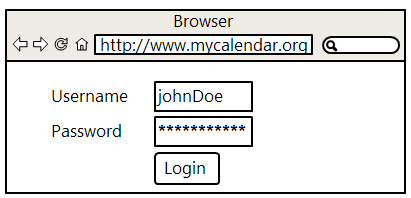
\includegraphics[width=0.8\linewidth]{Login.png}
	\caption{Wireframe model describing the Login screen.}
	\label{fig:login}
\end{figure}

\cref{fig:login} shows a wireframesketcher model of the login screen that has two text input fields and one button.
%TODO Quelle Ecore Metamodel
Wireframesketcher stores the models as instances of the Eclipse Ecore meta-model making it easy to integrate them with the domain-specific languages created for Feature and Mapping definitions.
After entering a valid username and a valid password the login can be executed by clicking the \textit{Login} button leading to the overview screen as shown in \Cref{fig:overview}.
The expected behavior for the Login screen is described formally within a Feature file that contains different scenarios.

\begin{lstlisting}[captionpos=b, caption=Feature Description: Login Screen., label={lst:featureLogin}, language=dsl]
Feature Login

As a "Calendar User"
I want to "login to the calendar application"
In order to "manage my appointments"

Scenario ValidLogin
Given I am on the Login screen 
when I type "johnDoe" in the Username textfield 
and I type "Password" in the Password textfield 
and I click the Login button
then I am on the the Overview screen
and the Appointments table is visible
\end{lstlisting}

\Cref{lst:featureLogin} shows the Feature description for the login screen that is divided into three main parts. 
The first part defines the feature name which in this case is \textit{Login}.
The name field is crucial for references to this file as well as for later generation and is therefore restricted to alphanumerical characters.
The second part of the feature definition contains the user story, that specifies the business value of the feature from the perspective of a certain user \cite{C.Solis.2011}.
The keyword sequences \textit{As a}, \textit{I want to}, and \textit{In order to} are predefined by the Specification Language grammar to ensure an uniform structure.
%TODO Quelle BDD Business Value of feature
Although, the second part is optional and therefore not evaluated by the generator it is an important mechanism to document that a feature has a business value (Quellen BDD).
%TODO Quelle gherkin
The third part describes different scenarios for each feature using grammar constructs that are a subset of the ubiquitous language gherkin enhanced by the functionality to connect to wireframe elements.
For a single feature there can be multiple scenarios within one file in order to describe different behavior of the screen.

The scenario in \Cref{lst:featureLogin} shows the description for a successful login.
The \textit{Login} scenario starts with the context area which sets a certain screen into focus that is thereby the starting point for following the command and assertion sections.
The first command starts with the keyword sequence \textit{When I} while all following commands in the same section begin with \textit{And I}.
The command introduced by the keyword sequence \textit{When I} is about typing the value ``\textit{johnDoe}" into the \textit{Username} textfield. 
Based on the screen in context the possible widgets, actions and their parameters are determined dynamically and proposed to the user while typing.
The \textit{When I} keyword sequences is proposed to structure the scenario description and the keyword \textit{type} is proposed dependent on the widgets on the screen in context.
The second part of the command determines on which widget the action should be executed.
At this point only such widgets are considered valid that are on the screen and applicable for the action keyword stated before.
Based on the underlying Ecore model, references can be validated at any time leading to early detection of scenarios affected by renaming or removing of widgets.
Thereby, potential errors within a test case can be determined before the test case has been executed.
The remaining two commands are concerned with entering the correct password before the \textit{Login} button is pressed.
The expected response of the application to the event triggered by clicking the button, is described in the next part of the scenario description.

The last part of the scenario description is the assertion section in which the screen content is checked after the commands have been executed.
The first assertion changes the screen context of the scenario, since it is assumed that after a successful login the \\begin{textit{Overview} screen is shown.
The following assertion statements introduced by the keyword sequence \textit{and the} are now executed in the context of the \textit{Overview} screen which means that only widgets from that screen can be referenced.

\begin{figure}[h]
	\centering
	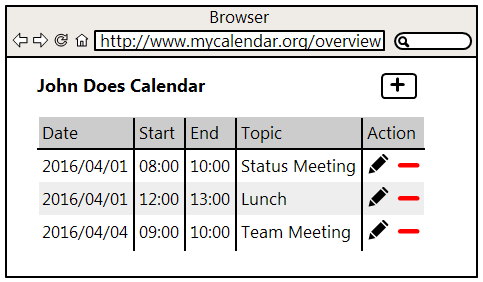
\includegraphics[width=0.8\linewidth]{Overview.png}
	\caption{Wireframe model describing the Overview screen.}
	\label{fig:overview}
\end{figure}

\Cref{fig:overview} Shows the Overview screen that is shown after a successful login and contains a table showing all known appointments and a plus button to add new entries.
To describe further scenarios for this screen a separate Feature description file is created.
After having created screen and Feature descriptions, a Mapping definition depicting the wireframe elements to their implementation is required to enable the generation of automated test cases.

\begin{lstlisting}[captionpos=b, caption=Mapping Description: Login Screen., label={lst:mappinglogin}, language=dsl]
Mapping Login

url {fragment:"#/login"}
label {nls{en:"Login"}}
Username{
	locator:"#username"
}
Password{
	locator:"#password"
}
Login{ 
    driver: org.sample.calendar.ButtonDriver
    locator:"#login"
}
\end{lstlisting}

\Cref{lst:mappinglogin} shows the Mapping description for the Login screen.
The first part of the file states the URL part needed to find the screen within the application which is ``\#/login". 
After the keyword \textit{label} the label of the application window, e.g. the browser window, is stated, which can be used for identifying and verifying the correct screen within the application.

The second part of the mapping files contains one entry for each widget on the screen.
As in the feature file, \textit{Username},\textit{Password}, and \textit{Login} are real references to the elements from the wireframesketcher model.
Since these can be validated feedback on the impact of changing a widget's or screen's name on the mapping files can be given early and automatically.
%TODO Quelle HTML DOM and IDs
For each widget there is one \textit{locator} which in case of a web application could be the ID of the element in the HTML document tree (Reference to HTML DOM).
For custom widgets or such that cannot be found using a simple ID mechanism a custom \textit{driver} can be specified as shown for the \textit{Login} button.
Explicitly stating a \textit{driver} will make the automated test try to find the widget using the custom \textit{driver}. 
The mechanism enables the use of custom widgets without applying any changes to the screen or feature description files.

The combination of screen, feature, and mapping file is used by the a generator to create a page object and a test script.
The first, encapsulates all interactions, such as clicking, typing, or resolving a label, per screen in a single class.
Basis for the page objects is the combination of screen and Mapping files.
For the example shown in \Cref{lst:featureLogin} there are two mapping files needed one for the \textit{Login} and one for the \textit{Overview} screen.
The second generation results are the test scripts that are generated using the information from the screen and feature files.
Every scenario is turned into a test method containing all actions and assertions from the Feature file.
%TODO Quelle Gherkin
The available default generator will create the test script in gherkin language optimized to be run with Cucumber and Selenium.
The page objects generated are simple groovy classes that encapsulate the interaction with the UI widgets.
%TODO Quelle SauceLab
Since the test scripts are based on the Cucumber framework they can be run locally, in a continuous integration environment or in a testing cloud such as SauceLab.

\subsection{Behavior-Driven UI Testing Architecture}
\begin{figure}[h]
	\centering
	\includegraphics[width=0.8\linewidth]{SpecificationLanguageArchitecture.png}
	\caption{Behavior-Driven UI Testing Architecture.}
	\label{fig:architectureOverview}
\end{figure}

\Cref{fig:architectureOverview} shows the architecture of the Behavior-Driven UI Testing approach divided into three logical parts. 
First, the Wireframesketcher model that contains the graphical editor as well as the underlying Ecore model used to reference screens and their widgets.
The functionality offered by Wireframesketcher tool has been re-used completely, however, some customizations were implemented as described in \Cref{sec:WireframesketcherIntegration}.

The Specification Language is divided into two logical parts namely the Feature and Mapping DSL.
The wireframesketcher model is used by the Feature and Mapping DSL component that encapsulate the grammar definitions and the the tooling implementation to support context-sensitive proposals, validations and syntax highlighting.
As shown in \Cref{fig:architectureOverview} Feature and Mapping DSL are completely independent from each other.
Thereby, it is possible to use Wireframesketcher and the Feature DSL to concisely define requirements without taking advantage of generating any automated test cases.
Further, it is possible to only generate the page objects from the combination of Wireframesketcher model and Mapping DSL and implement the test cases manually.

As shown in \Cref{fig:architectureOverview} both generator implementations are independent and separated from the domains-specific language modules.
Thereby, generators can be switched at runtime to generate for different environments, such as web or Eclipse RCP applications, without changing the DSLs.
Both generators interact with the wireframesketcher model as well as with the respective domain-specific language definition.
The following sections will explain the modules content and their interaction in more detail.

\subsection{Wireframesketcher Integration}\label{sec:WireframesketcherIntegration} 
%TODO Quelle Wireframesketcher
Wireframesketcher is an tool for creating UI descriptions for GUI based applications. 
It is well integrated in the Eclipse toolchain and offers many different UI styles, such as SWT, iOS, and HTML5.
%TODO reference to repository
The sketches are stored in an Ecore model that is available in an open source repository.
To use wireframesketcher models as basis for Feature and Mapping descriptions that underlying Ecore model was enhanced.

First, the existing marker interfaces, such as ClickSupport and SelectionSupport, were enhanced to support more advance concepts such as DoubleClickSupport and BooleanSelectionSupport.
Based on the marker interfaces implemented by a widget the proposal of available actions within a scenario description are determined at runtime.
Second, the Screen class was extended to hold a \textit{name} attribute that is needed to create references to it from a feature or mapping definition.
%TODO Reference to ResourceDescriptionStrategy
Finally, the ResourceDescriptionStrategy of the wireframesketcher model was extended to work with nested elements on a screen, such as widgets in containers or widgets in tables.

The adjustments described above extend the capabilities of the underlying model, but had no side-effects on the remaining wireframesketcher tooling for drawing sketches.
%TODO Quelle Feature Patch
The model adjustments are delivered as an Eclipse feature patch that is fully inter operable with the wireframesketcher UI functionalities so that they can be reused to create wireframe models.

In order to support more complex UIs that are composed from different application parts, wireframesketcher supports reusable components.
%TODO Link zu Wireframe Components explanation
These components are defined as screen files, however, they are marked within wireframesketcher as components and thereby become reusable for other screen files.
These components are very handy when for example defining a screen that is divided into different tabs.
In that case the tabbed pane on is defined as reusable component and each tab is defined as one screen file.
Thereby, the common part which is the tabbed pane and all the widgets on it, e.g. shared buttons or labels, are factored out.

The additions made to wireframesketcher as well as the already existing functionalities allow users to define sound and comprehensive UI descriptions. 
Furthermore, storing the wireframe models as Ecore meta-model instances enable the integration into the Xtext based Feature and Mapping DSL as the following sections will illustrate.

\subsection{Feature DSL}
\subsubsection{Basic Grammar}
The Feature DSL is the central part of the Specification Language defining the general structure of the document as well as the available keyword sequences.
The structure of a feature file as described in \Cref{sec:SpecifyingTheApplication} consists of three main parts.
The first part holds the feature name and an import section for the used screens and widgets.
The second part holds the user story given the benefit of the described feature from a specific user role.
The third and most important part hold an arbitrary number of scenario descriptions for the feature file.

%TODO Is this really needed? Does not contain many interesting constructs
%TODO Add grammar for assertions
%TODO Add annotations
\begin{lstlisting}[captionpos=b, caption=Feature Grammar, label={lst:featureGrammar}, language=xtext]
Scenario:
'Scenario' name=StringOrId
GivenIamOnThe toScreenSwitch=ToScreenSwitch 
codeStatements+=CodeStatement*;

CodeStatement:
(AndI | WhenI ) AbstractCommand | 
(AndThe | ThenThe | ThenIt ) Assertion |   
ThenIAmOnThe ToScreenSwitch;

AbstractCommand:
Command|ImplementedCommand;

Command:
action=Action InThe widget=WidgetWrapper;

Action:
ClickAction |TypeAction;

ClickAction:
{ClickAction}
'click';

TypeAction:
'type' value=StringOrParam;
\end{lstlisting}

\Cref{lst:featureGrammar} shows a part of the Feature Grammar that is basis for the definition of the scenario described in \Cref{lst:featureLogin}.
After setting the name, the scenario description continues with setting the context to a specific screen before the commands and assertions are defined.
As shown above an \textit{Command} consists of an actual action such as ``click" or ``type" that is followed by the widget on which it should be applied.
Actions may have parameters for example to specify what should be typed into a text field. 
In addition, there are \textit{Assertion} statements that define the third part of a scenario description containing the expected outcome of an \textit{Command}.
Within a scenario it is possible to mix both kinds of statements so that one scenario could describe a series of commands and assertions, e.g. for larger processes taking place on a single or multi screen application.   

\subsubsection{Advanced Concepts}
In addition to the capabilities shown so far the Feature DSL supports advanced concepts such, external test data, composed test cases, manually implemented commands and assertion and integration with state of the art Application Lifecycle Management tools.
 
The first advanced concept deals with integrating external test data into the Feature definition by introducing ``parameters" and ``data providers".
Parameters can be used as placeholders instead of concrete text, e.g. in the \textit{BTypeAction} rule from \Cref{lst:featureGrammar}.
Within the genarated test cases the data provider is asked to replace the parameter by an actual value.
A data provider can be bound to a scenario using the Data Provider annotation that has to reference a class implementing the \textit{DataProvider} interface.
Parameters and data providers separate the Feature specifications from the actual test data and thereby make them more resilient and also executable with different test data sets.

The second advanced concept introduces dependencies between scenario definitions to the grammar.
Although it is considered good practice to keep test cases independent from each other, there are situations in which a certain chain of actions is required by multiple test cases.
In the calendar application for example the tests of the edit functionality will all start with selecting an existing entry from the table of already created appointments.
Within the Feature DSL this particular part of selecting an entry from the table and clicking the edit button can be factored out to an reusable scenario.
To re-use such a scenario the Feature DSL offers a ``depends on" Annotation that can be added to each scenario and holds a reference to a reused scenario.
Based on this information the generator will generate the reusable code into the annotated scenarios test method, so that the test methods depend on each other logically, but remain independent on the source level.

Another advanced concept of the Feature DSL are \textit{ImplementedCommand} statements that can be used to specify custom behavior, e.g. setting the content of a custom widget.
Within the grammar the \textit{ImplementedCommand} is a simple String, but during generation it is turned into a test method that needs to be implemented manually. 
Besides \textit{ImplementedCommands} there are also  \textit{ImplementedAssertion} that can be used within a scenario definition to define manually implemented assertions.
Although, one of the main goals of the introduced approach is to provide fully generated automatically executable test cases, there are situations in which a manual implementation is required. 
However, manually implemented commands and assertion are a good basis for extending the Feature and Mapping grammar in order to support more advanced concepts and to get rid of manual implemented and maintained code.

Finally, since test cases and their results are usually managed within a test management tool, e.g. HP Quality Center or SAP Solution Manager, the Feature DSL offers a connection to these systems.
In the first implementation a connector for the HP Quality Center software has been included that leverages the REST API of HP Quality Center.
To connect to the HP Quality Center a configuration files needs to be provided holding basic information, such as URL, test project name and credentials.
In addition, every scenario can be enhanced with a Annotation stating the HP Quality Center ID of the respective test case.
Whenever a test is executed and a connection is configured the result is stored in HP Quality Center.
By integrating a HP Quality Center the tests can not only be automatically executed, but are also tracked in a application lifecycle management system allowing for detailed analysis and reports.


\subsection{Mapping DSL}
The main advantage of the introduced approach is that it allows to generate automatically executable test cases.
The basis for this innovation is on the one hand the integration of wireframesketcher models and on the other hand the Mapping DSL.
The latter is required to map the logical elements within a wireframesketcher model such as \textit{Screen} or \textit{Widget} to their implementation.
As shown in \Cref{lst:mappinglogin} mapping files are defined per \textit{Screen} and consist of two parts.
The first holds the name of the mapped screen and an ``url" attribute containing a relative URL to find the screen within the application.
In addition, a ``label" attribute can be specified to verify that for example in an web application the name of the browser window matches the label.
The second contains the mapping information for all widgets on the particular \textit{Screen}.
The widget mappings consists of a reference to the wireframesketcher model element, the ``locator" attribute, and an optional ``driver" attribute.
The locator attribute is a String value that exactly identifies the widget within the screen.
For a web application this might be the ID of an element in the DOM tree.
The optional driver attribute holds a String value that represents a class on the classpath of the test project that is used interact with the widget.
Specifying a custom driver allows to use custom widgets and their custom functions, e.g. to identify them.

Since their is deep knowledge about the implementation necessary to fill out the mapping file, it should be created and maintained by the responsible developer. 
Because developer availability is usually very limited especially when it comes to writing tests, the introduced approach tries to reduce developer involvement.
First, this is achieved by having one mapping file per Screen that is separated from the actual test description, so that the mapping definition is structured in known chunks (Screens in this case). 
Second, the references to the EClasses representing the wireframesketcher widgets allows for extended validation support, e.g. automatically checking if all widgets of a screen are mapped.
Finally, the reusable component feature of wireframesketcher is copied by the mapping DSL, so that reusable screens only have to be mapped once.

\subsection{Generator}\label{sec:Generator} 
After having defined wireframesketcher, feature and mapping descriptions a generator turns the three files into automatically executable test specifications.
As shown by \Cref{fig:architectureOverview} there are two kinds of generators that are loosely coupled to the DSLs and the wireframesketcher model.
The default implementation is a generator for web applications, that generates Cucumber specification files.
In addition, there has been a proprietary generator for an SWT based RCP application.
Since the feature and mapping files are created within Eclipse projects the generator to use can be defined per project.
Within the properties of an Eclipse project any generator that is registered through the Eclipse Extension mechanism can be selected.
Before a generation starts, the application asks the Property Service which generator should be executed and then tries to find that generator within the registered extensions.
Being able to change the generator at such a late stage makes the whole approach very flexible, however, it also adds restrictions to the DSLs.
To allow changing generators lately the DSLs need to be generic to a level that different UI applications such as web, SWT or Swing based can be described.
In addition, the DSLs should support the requirements engineer during the creation of test specfications by giving reasonable proposals.

%Fowler: Page Objects
In order to interact with the widget on a screen, the mapping generator create an Page Object [Quele Fowler] per Screen file.
Within these page objects all interaction with the screen and its widgets are encapsulated.

\begin{lstlisting}[captionpos=b, caption=Generated Page Object, label={lst:MappingGenerated}, language=dsl]
class LoginScreen {
	static url = "#/login"
	static at = { waitFor { title == "Login" } }
	
	static content = {
		username (required: true) { module org.boomslang.module.BoomslangModule, $("#username") }
		password (required: true) { module org.boomslang.module.BoomslangModule, $("#password") }
		submit (required: true , wait:true) { module org.sample.calendar.ButtonDriver, $("#login") }
	}
}
\end{lstlisting}

\Cref{lst:MappingGenerated} shows the page object for the Login example that is generated as groovy file.
The page object is in Groovy programming language because it interacts well with the Cucumber test specification that is generated by the Feature generator.
The structure of the generated page object is very close to the Mapping file because in the end the Mapping DSL is just an slightly enhanced page object description.
The main part of the screen is the ``contentW attribute that holds the locators for all the widgets on the screen.
If a ``driver" is specified in the Mapping file, it is referenced here and during runtime of the test cases the Cucumber driver tries to find the class on the classpath.

\begin{lstlisting}[captionpos=b, caption=Generated Feature File, label={lst:featureGenerated}, language=dsl]
	def "ValidLogin"() {
	given:
	to (org.specification.calendar.LoginScreen);
	
	when:
	username.value $username
	and:
	password.value $password
	
	then:
	at OverviewScreen
	and:
	waitFor { appointments }
	
	where:
	$password | $username
	"Password" | "johnDoe"
}
\end{lstlisting}
Although the Feature Generator is logically separated from the Mapping generator it relies on the page objects.
Within the generated Cucumber specification the page objects are instantiated and used to interact with the application.
\Cref{lst:featureGenerated} presents the generated cucumber test script for the Login example. 
Like the page object the test script's structure is very close to the feature file it is generated from.
This is due to the fact that the Feature DSL itself introduces no new concepts to the general structure of a feature or scenario description.
The invention lies in the connection to the page object that is fully generated and therefore makes the test script ready to be executed without any further manual adjustments.
One small enhancement compared to the feature file is in the ``where" section that holds the data used in the test scenario.
This section is a feature of the underlying Cucumber framework that enable the test to run with different data input. 
The test case will be executed for each line of data, so that this way of generating makes it easy to run the same script multiple times with different test data.

Since the test cases can be executed without further manual interaction the generator can be included in a continuous integration environment.
Whenever the application under test is builded the test generator is called to turn feature and mapping files into test specifications before these are executed during a the build.
By integrating the generator into the development process the basic principle of test driven development, specify test, fail, implement, pass can be ensured.


\section{Discussion}\label{sec:Discussion}
The introduced approach extends the well-known and industry proven methodology of behavior-driven design to enable fully generated automated test cases.
By combining wireframes and feature definitions test case creation can be supported by enhanced editing and validation mechanism.
The first implementation supports basic widgets such as text fields, buttons, and tables, however, there are more standard widgets such as tabbed panes or accordeon panes that should be supported by future versions.
Besides being able to handle custom widgets using implemented commands, and assertions, and custom drivers, it is to be discovered which widgets are to be supported by the default.
With the flexible architecture of the introduced approach it is possible to support all kinds of custom widgets from wireframe through feature and mapping file up to the generator.

Since the approach focuses on increasing the productivity and the test coverage of software developing project, the Specification Language can be integrated into the whole process.
Feature specification and wireframes are created and maintained within an Eclipse project that can be checked in together with the source of the application.
The generated test cases do not need to be managed by a source code management system such as git or svn, since they can be completely generated.
The tooling to generate and execute test cases can be introduced at different stages within the development process. 
First, the generator can be triggered locally as part of a maven build to generate and run the tests locally.
Second, the same generator can be called during the build of the application under test to execute the test cases within an continuous integration environment.
Finally, the results of every test run can be stored in professional lifecycle management Systems like HP Quality Center.

The introduced Specification Language has been tested within the development of an application in the financial sector. 
The developed application consist of two components, where one is a web application and one is SWT application.
While the first is supporting the bank advisor in the process of analyzing the financial situation of the client, the second focuses on backoffice tasks to actively manage client portfolios.
The advantage of using wireframesketcher was that both wireframe models were instances of the same meta-model so that they both could be integrated into the Feature and Mapping DSL, although, the graphical representation was slightly different.
In addition to using the same wireframesketcher meta-model it was proven possible to use the same Feature and Mapping DSL to describe the behaivor and and the widget mapping of both applications.
Since the web-application was tested using Cucumber and gherkin the SWT application was tested using SWTBot, therefore, two generators where implemented.
One disadvantage of introducing the specification language to the development process is the large number of technologies involved.
To completely integrate into the process a variety of frameworks is needed such as Xtext, Cucumber, Maven, Selenium.
Besides solely including these technologies they all require a certain amount of knowledge to configure all parts consistently and to fully leverage the potential of the specification driven approach.

Within the projects that used the Specification Language wireframesketcher was already known as well as JBehave for defining feature descriptions.
As a consequences the Specification Languages was adapted very quickly by requirements engineers and developers, because it was not introducing a new tool or technique, but bringing existing approaches together.
Furthermore, in contrast to JBehave the involvement of developers in the process of writing tests was decreased by 75\% limiting their efforts only to providing the mapping definitions.
The feedback from requirements engineers was specially emphasizing the advanced validation possibilities that helped to keep wireframes and requirements specifications congruent.

%TODO Find the sweet spot of generation. Not generated 100%, but generate 80 and allow the remaining 20 to be manually implemented fast and easy


\section{Conclusion}\label{sec:Conclusion} %and Future Work
The specification Language introduced by this paper combines the ubiquitous BDD language with wireframesketches to fully generate automated test cases.

In many projects requirements engineers or architects are heavily involved in the task of defining services and their input output parameters.
However, the description is often only a textual description of the input and output parameter and potential exceptions. 

%TODO More commands and actions like table, trees and lists that can be elaborated in more detail 

%TODO Future work: How to compose tests scripts for UI comming from different components? First expecting every component to deliver a tested UI, but who is repsonsible for integrated tests and where should they be managed?

%\newpage
%
% The following two commands are all you need in the
% initial runs of your .tex file to
% produce the bibliography for the citations in your paper.
%IMPORTANT directly embedded
\bibliographystyle{abbrv}
\bibliography{specification_driven_testing}  % sigproc.bib is the name of the Bibliography in this case

%\begin{thebibliography}{10}
%\end{thebibliography}

% You must have a proper ".bib" file
%  and remember to run:
% latex bibtex latex latex
% to resolve all references
%
% the ACM needs 'a single self-contained file'!
%
%\balancecolumns
\begin{comment}
\appendix
%Appendix A
\section{Headings in Appendices}
\subsection{References}
Generated by bibtex from your ~.bib file.  Run latex,
then bibtex, then latex twice (to resolve references)
to create the ~.bbl file.  Insert that ~.bbl file into
the .tex source file and comment out
the command \texttt{{\char'134}thebibliography}.
%\balancecolumns
\end{comment}
\end{document}
